\documentclass{elsarticle}
\usepackage[margin=2.5cm]{geometry}
\usepackage{CJKutf8}
\usepackage{lineno}
\usepackage[colorlinks=true,
           urlcolor=blue,
           citecolor=blue,
           linkcolor=blue,
           % bookmarksopen,
           % bookmarksopenlevel=1,
           % pdftitle={},
           % pdfauthor={Joe Doe},%
           % pdfsubject={},%
           % pdfkeywords={provenance, workflows},
           bookmarks=false,
           bookmarksnumbered,% For PDF navigation
           % backref=page,
           % pagebackref=page,
           linktocpage=true
           ]{hyperref}
\usepackage{color}
\modulolinenumbers[5]
\journal{, homework for Academic Writing}%这里可以修改首页页尾
\newif\iffinal
% Un-comment this line to see proposal without comments
\finaltrue

\definecolor{olive}{rgb}{0.5, 0.5, 0.0}
\iffinal
  \newcommand\change[1]{}
  \newcommand\kyle[1]{}
  \newcommand\victoria[1]{}
  \newcommand\kacper[1]{}
  \newcommand\mihael[1]{}
\else
  \newcommand\change[1]{{\color{blue}[Change: #1]}}
  \newcommand\kyle[1]{{\color{blue}[Kyle: #1]}}
  \newcommand\victoria[1]{{\color{red}[Victoria: #1]}}
  \newcommand\kacper[1]{{\color{green}[Kacper: #1]}}
  \newcommand\mihael[1]{{\color{olive}[Mihael: #1]}}
\fi

%%%%%%%%%%%%%%%%%%%%%%%
%% Elsevier bibliography styles
%%%%%%%%%%%%%%%%%%%%%%%
%% To change the style, put a % in front of the second line of the current style and
%% remove the % from the second line of the style you would like to use.
%%%%%%%%%%%%%%%%%%%%%%%

%% Numbered
%\bibliographystyle{model1-num-names}

%% Numbered without titles
%\bibliographystyle{model1a-num-names}

%% Harvard
%\bibliographystyle{model2-names.bst}\biboptions{authoryear}

%% Vancouver numbered
%\usepackage{numcompress}\bibliographystyle{model3-num-names}

%% Vancouver name/year
%\usepackage{numcompress}\bibliographystyle{model4-names}\biboptions{authoryear}

%% APA style
%\bibliographystyle{model5-names}\biboptions{authoryear}

%% AMA style
%\usepackage{numcompress}\bibliographystyle{model6-num-names}
\usepackage{fancyhdr}
\pagestyle{fancy}
\rhead{written by LaTex.}

\begin{document}
	
\begin{frontmatter}

%Capturing the ``\wt\ '' of Computational Claims: 
\title{\textbf{Service Revolution: Has the Mobile Internet\\Upgraded the Traditional Services?}}
% \tnotetext[mytitlenote]{Fully documented templates are available in the elsarticle package on \href{http://www.ctan.org/tex-archive/macros/latex/contrib/elsarticle}{CTAN}.}

%% Group authors per affiliation:
%\author{Bertram Ludaescher\fnref{myfootnote}}
%\address{School of Information Sciences, University of Illinois at Urbana-Champaign}
%\fntext[myfootnote]{School of Information Sciences, University of Illinois at Urbana-Champaign}

%% or include affiliations in footnotes:
%\author[mymainaddress,mysecondaryaddress]{Elsevier Inc}
%\ead[url]{www.elsevier.com}
\author{Xiwen Lu\fnref{fn,fn1}}%(\url{luxiwen@cumt.edu.cn})
\address{School of Computer Science and Technology, China University of Mining and Technology}
\ead{luxiwen@cumt.edu.cn}

\fntext[fn]{Class, 6}
\fntext[fn1]{NO, 03170908}


\begin{abstract}
Mobile Internet started to emerge 10 years ago, and with the development of recent years, it has gradually brought a huge impact on all aspects of people's traditional life.This paper selects the aspects of "shopping", "travel" and "entertainment" closely related to daily life to analyze the impact of mobile Internet on traditional service industry.The herd effect theory is cited to further analyze the impact.Finally, combined with specific data, the prediction accuracy of herd theory on the impact of traditional industries was demonstrated.Finally, the direction of hot spots in the next Internet stage is proposed for the future. 
\end{abstract}


\begin{keyword}
\texttt{mobile internet \sep herd effect \sep online shopping \sep mobile travel \sep short video}
%\MSC[2010] 00-01\sep  99-00
\end{keyword}
\end{frontmatter}

\begin{CJK}{UTF8}{song}

\noindent\textbf{摘要}\\
\indent \ \ 移动互联网10年前开始兴起,随着近几年的发展,逐渐对人们传统生活的各个方面带来了巨大的影响。本文选取了与日常生活息息相关的“购物”、“出行”、“娱乐”方面,分析移动互联网对传统服务行业的冲击。援引羊群效应理论,进一步分析冲击所产生的原因与影响。接着,分析泛移动互联网对社会和个人的潜在危害。最后,面向未来提出移动互联网的新展望并对全文进行总结。\\
\\
\textsl{关键词:}\ \ 移动互联网,羊群效应,网上购物,移动出行,短视频

%\twocolumn[]
\end{CJK}

%\linenumbers
\section{Introduction}\label{sec:intro}

\subsection{Mobile Internet}
Thanks to the advent of smart devices and the emergence of 3G/4G wireless technologies, services over mobile phones are becoming in many respects similar to those available over the PC based internet. Indeed mobile web-based services, such as search, maps, presence, messaging, emails, productivity, social networking, and entertainment are becoming available in high-end phones from several device manufacturers~\cite{hlw3,hlw8}. Mobile computing, however, promises richer applications and services based on location and context. Web technologies are being adapted and extended to support emerging mobile internet services. However, location based mobile services present new significant challenges in terms of implementation and management complexity. In this presentation we will discuss the business trends of mobile services. Through a discussion of current projects at IBM Research, we will also present examples of the technology trends supporting scalable location based services~\cite{MSBTT,MSBTT2,MB}.


\subsection{Traditional Services} 

The traditional service industry is now faced with the information asymmetry between service providers and users, and service providers are in the dilemma of high competition, high advertising, high investment and low benefit for a long time~\cite{hlw,hlw2,hlw7}.On the contrary, users often cannot get help through search engines, classified websites and other means, and a series of challenges brought by consumption upgrading are also imminent.

\subsection{Transformation of Services Industry}
With the development of information technology and knowledge economy, the traditional service industry will be transformed with modern new technologies, new forms of business and new services to create demand, guide consumption, and provide the society with high value-added, high-level, knowledge-based production services and life services.
The development of modern service industry essentially comes from the demand of social progress, economic development and specialization of social division of labor~\cite{cx,cx4,cy}.It has the characteristics of high concentration of intellectual elements, high added value of output, less consumption of resources and less environmental pollution.Modern service industry includes both the emerging service industry and the technical transformation and upgrading of the traditional service industry. Its essence is to realize the modernization of the service industry.\\


The remainder of this article is structured as follows. In Section~\ref{sec:relatedwork} we first
present some work that other scholar studied about some of the innovation of tradition service industry. In Section~\ref{sec:inno} we choose three important aspects in daily life to analyse the innovation of traditional services industry(i.e. shopping, travelling, enjoyment). Then, we cite ``herd behavior'' to analyze the impact of mobile Internet on social lifein Section~\ref{sec:herdeffect}. Last but not least, in Section~\ref{sec:harm} we analyzes the potential harm of the rapid development of mobile Internet from two perspectives of society and individuals. Finally, we summarize our contributions
in Section~\ref{sec:summary}.

\section{Related Work}\label{sec:relatedwork}
Mobile Internet plus is increasingly becoming a topic of widespread concern. Many aspects of social life have attracted the addition of Internet elements, and many scholars have also noticed this and done a lot of research on these shoots of bamboo shoots after rain. For example, Online shopping~\cite{wg,wg7,wg8,wm2}, online payment\cite{wm,jr,jr2}, Internet travel\cite{che,che3,che4}, information construction library\cite{chm,tsg}, short video\cite{dsp,dsp3,dsp7}, Internet social networking\cite{hlw}. 

\begin{figure}[ht!]
	\centering
	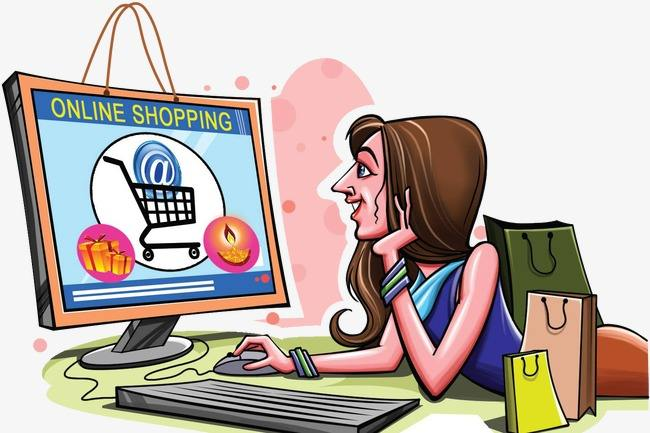
\includegraphics[trim=0in 0in 0in 0in,clip,width=0.75\columnwidth]{onlineshopping.jpg}
	\caption{Shopping on the Internet has become a favorite shopping way of young people.
		\label{fig:on_shop}}
\end{figure}

Mobile Internet has a profound influence on human society and really promotes the formation of networked society.The "personalized" needs of individual users converge to form a new world with "group" characteristics\cite{SSMSO,DBLP}.These groups have distinct characteristics that will drive the continuous development of technology and applications\cite{extend}.The mobile Internet can efficiently meet people's "fragmented" needs at different times and places through the network platform, which are often new niche needs that traditional industries cannot meet or have never met.

\section{Innovation}\label{sec:inno}
We first describe three scientific domains that, like many others. We 
focus specifically on examples that elucidate the innovation. 

\subsection{Online Shoping}
Shopping on the Internet, is through the Internet to retrieve commodity information, and through the electronic purchase order issued shopping request, and then fill in a personal check account or credit card number, manufacturers through mail order delivery, or through the express company home delivery.

\begin{itemize}
	\item \textbf{for consumers:}
	Can "shop around" at home, ordering without time, place restrictions;Obtain a lot of commodity information, can buy local products;Online payment is safer than traditional cash payment to avoid cash loss or robbery.
	
	\item \textbf{for merchants:} Due to online sales inventory pressure, low operating costs, operating scale is not limited by the site.In the future, more enterprises will choose online sales and adjust their business strategies through timely feedback of market information through the Internet, so as to improve their economic benefits and their ability to participate in international competition.
	
	\item \textbf{for the whole market money:} This new shopping mode can realize resource allocation in a larger scope and a wider level with higher efficiency.To sum up, online shopping has broken through the barriers of traditional commerce and has great appeal and influence on consumers, enterprises and the market. In the new economic era, it is undoubtedly an ideal model to achieve the "all-win" effect.
	
\end{itemize}

\subsection{Mobile Travel}
Online car-hailing refers to the way to travel by building a service platform based on Internet technology and realizing point-to-point transportation services by using smart phone application software to reserve vehicles.With the help of Internet platform and large data technology, online car hailing greatly reduces the cost of information acquisition and transaction cost, which challenges the economic control theory of traditional taxi.The advantages of online car hailing are as follows\cite{che,che3,che4}.\\

The emergence of online car hailing has many benefits. First, the high information transparency greatly changes the problem of information asymmetry.Second, there is sufficient market competition and good positive externalities.


\subsection{Enjoyment}
Take \emph{short video} as example. Different from the previous one-way communication of mass media, information transmission has a feedback time difference.In the process of network communication, the communication mode between information disseminator and information receiver presents the characteristics of two-way feedback.The communication characteristic of two-way feedback depends on the interaction of information transmission and receiving, that is, the interaction between information creators, disseminators and audiences.Audiences can comment and share video content on social platforms.\\

In addition, in the aspect of knowledge acquisition, taking the informatization construction of university library as an example, many scholars have carried out research and explored more diversified ways to carry out the information construction of library\cite{tsg,chm}.\\

Finally, the emergence of mobile Internet has greatly changed the traditional way of service, and its influence can be seen in every aspect of people's life.In the near future, more new rules will be created by the mobile Internet in the service industry, and more old rules will be broken~\cite{zw10}.

\section{Herd Effect}\label{sec:herdeffect}
Herd behavior is a widespread social phenomenon. Initially, it was mainly used to study user behavior in financial market and software market, and later it was extended to the field of information system.

For example, in Internet shopping section, there are many sellers and different kinds of goods and abundant in quantity, a variety of promotional activities emerge in endlessly consumption. People often lack enough knowledge, time and energy to compare and contrast Analyze which product or service is better, so consumers buy less The uncertainty of the object will imitate others to carry out shopping, thus producing impact Moving the shopping behavior\cite{wgheyang}.

\subsection{Definition}\label{sec:defi}
In the study of consumer behavior, herding effect mainly refers to the cause
Consumers' personal information is not complete and is subject to other information in shopping
People shopping decision to follow the influence of other consumers shopping
Behavior.Herd behavior mainly refers to behavior decision-making process
People imitate others and do not exactly what they originally intended
The phenomenon of decision making.Bikhchandani et al. believe that herd behavior requires two conditions: correct decision makers ``Incomplete personal information" and ``observing previous decisions" means ``imitating him the power of man".Thus it can be seen that the external influence as well as the individual. Under the premise of incomplete information, it is easy to lead to herd behavior and follow him. It can be seen from the \emph{Image}, which represents the \emph{herd effect} (see Fig.~\ref{fig:herdeffect}).


\begin{figure}[ht!]
	\centering
	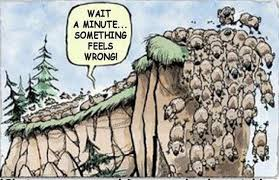
\includegraphics[trim=0in 0in 0in 0in,clip,width=0.75\columnwidth]{herdeffect.jpg}
	\caption{In the era of mobile Internet, herd behavior is reflected in people's eagerness to try new things.\label{fig:herdeffect}}
\end{figure}


\subsection{Performance}

With the development of e-commerce, herding effect has been further extended to network shopping behavior research. Chen confirmed that network shopping has obvious herding effect, and consumers will follow other consumers to buy books under the influence of other consumers' information recommendation.Xu et al. took the "double eleven" shopping situation of alibaba as the research object, and demonstrated that during the "double eleven" period, consumers, influenced by others, imitate others to produce herd effect and influence consumers' shopping behavior~\cite{wgheyang}.During shopping, consumers can obtain shopping information by talking with others and understand their shopping behaviors through observation. All these will affect consumers' shopping behaviors, indicating that there is a herd effect during shopping, and consumers will follow others to purchase.


\section{Potential Harm}\label{sec:harm}

\subsection{to the society}
The rapid development of China's mobile Internet has not only brought changes to the communication ecology and information industry pattern, but also triggered changes in China's economy, politics, society, culture, news communication and other fields, which has brought all-round influence to Chinese society.

\begin{enumerate}
	\item For China's development, accelerate social transformation and add impetus to development;To economic life, build intelligent network, change marketing concept.
	\item For political life, everyone has a wireless microphone to "participate in politics and discussion" anytime and anywhere.
	\item For news communication, accelerate the transformation of communication mode and change the pattern of media industry.
	\item For cultural life, unlimited learning and creative space, rich cultural consumption and enjoyment.
	\item For human civilization, a more transparent and open highly informationized society is coming.

\end{enumerate}


\subsection{to the individual}
With the further development of mobile Internet, more jobs will be integrated.The division of labor in society is further refined, and fewer people are needed to complete the same work.For every individual, it is hard not to be affected by the mobile Internet. Many teenagers will also be affected by Internet addiction and become more isolated.These dangers are not to be underestimated.

\begin{figure}[ht!]
	\centering
	
\includegraphics[trim=0in 3in 0in 0in,clip,width=0.75\columnwidth]{caiyuan.png}
	\caption{In the era of ``Mobile Internet", social division of labor is further refined, resulting in a large number of unemployment.\label{fig:caiyuan}}
\end{figure}


In the era of mobile Internet,
The most obvious feature is increased information feedback
Link, "transmission - feedback" with the help of new media
The platform also realizes interpersonal communication across time and space
And mass communication, enabling new media empowerment
The later receiver of the message becomes the sender of the message at the same time\cite{zw10}
The unity of the two identities awakens the strong
Self-consciousness, so that "transmission - feedback" no longer
Pay attention to whether the information is true, but enjoy the participation
And its pleasure, directly past the "gatekeeper"
As a result, rumors spread on the Internet
Meaning.



\section{Summary}\label{sec:summary}
Mobile Internet business model diversification.A successful business needs a successful business model to support it.The new characteristics of mobile Internet services provide space for business model innovation.With the development of mobile Internet into the fast lane, the network, terminal, users and other aspects have laid a solid foundation, unprofitable situation has begun to change, mobile Internet has been integrated into the mainstream life and business society, monetization wave is coming.Mobile games, mobile advertising, mobile e-commerce, mobile video and other business models flow liquidity quickly improved.\\

Big data mining into a blue ocean, precision marketing potential highlights.With the rapid improvement of mobile bandwidth technology, more sensor devices and mobile terminals can access the network anytime and anywhere, and driven by cloud computing, Internet of things and other technologies, China's mobile Internet has gradually entered the era of "big data".At present, the field of mobile Internet is still focused on precision marketing of location. However, with the development of big data related technologies and the deepening of data mining, customized application services and marketing methods for users will become a development trend, which will be another blue ocean of mobile Internet.

\begin{CJK*}{UTF8}{gkai}

\section*{References}

\small
\nocite{*}
\bibliographystyle{elsarticle-num}
%\bibliographystyle{alpha-initials-big}
%%%%%%%%%%%%%%%%%%%%%%%
%\bibliography{references}
\bibliography{references_ch}	
	
\end{CJK*}


\end{document}